\documentclass[twoside,11pt]{article}

% Any additional packages needed should be included after jmlr2e.
% Note that jmlr2e.sty includes epsfig, amssymb, natbib and graphicx,
% and defines many common macros, such as 'proof' and 'example'.
%
% It also sets the bibliographystyle to plainnat; for more information on
% natbib citation styles, see the natbib documentation, a copy of which
% is archived at http://www.jmlr.org/format/natbib.pdf

\usepackage{jmlr2e}
\usepackage{lipsum}
\usepackage{amsmath}
\usepackage{hyperref}
\usepackage{algorithm,algorithmic}
\usepackage{soul} % highlight
\usepackage{xcolor}
\usepackage{listings}

\lstdefinestyle{mystyle}{
    backgroundcolor=\color{gray!5},        % Very very light gray background
    basicstyle=\ttfamily\scriptsize,      % Typewriter font with smaller size
    commentstyle=\color{gray},            % Comment color
    keywordstyle=\color{blue},            % Keyword color
    stringstyle=\color{red},              % String color
    breaklines=true,                      % Automatically break long lines
    frame=single,                         % Draw a frame around the code
    rulecolor=\color{lightgray},          % Frame color set to light gray
    showspaces=false,                     % Don't show spaces
    showstringspaces=false,               % Don't show spaces in strings
    showtabs=false,                       % Don't show tabs
    tabsize=4                             % Set default tab size
}

\setcitestyle{square}

% Definitions of handy macros can go here

\newcommand{\dataset}{{\cal D}}
\newcommand{\fracpartial}[2]{\frac{\partial #1}{\partial  #2}}

\renewcommand{\algorithmicrequire}{\textbf{Input:}}
\renewcommand{\algorithmicensure}{\textbf{Output:}}

% Heading arguments are {volume}{year}{pages}{submitted}{published}{author-full-names}
\jmlrheading{}{2024}{}{}{}{Griffon, Smoliakov, Yntykbay}

% Short headings should be running head and authors last names

\ShortHeadings{Predicting Air Pollution Levels in India}{Griffon, Smoliakov, Yntykbay}
\firstpageno{1}

\begin{document}

\title{Predicting Air Pollution Levels in Five Major Indian Cities}

\author{\name Aleksandr Jan Smoliakov \email aleksandr.smoliakov@mif.stud.vu.lt \\
  \name Danial Yntykbay \email danial.yntykbay@mif.stud.vu.lt \\
  \name Davide Giuseppe Griffon \email davide.griffon@mif.stud.vu.lt \\
  \addr Data Science study programme\\
       Faculty of Mathematics and Informatics}

\editor{Jurgita Markevi\v{c}i\={u}t\.{e}}

\maketitle


\begin{abstract}

  Air pollution ranks among the most pressing global health threats, causing an estimated 3 to 9 million deaths annually.
  India, with its rapid urbanization and economic growth, faces some of the highest pollution levels globally. The country's air pollution stems from a combination of natural and anthropogenic sources, emitting harmful pollutants such as carbon monoxide (CO) and particulate matter (PM\textsubscript{10} and PM\textsubscript{2.5}).

  This project aims to develop a predictive model for air pollution levels using a multivariate regression approach. The model will incorporate a wide array of predictors, including geographic location, seasonal variations, meteorological data and temperature. By evaluating various modeling techniques—starting with linear regression and potentially expanding to more complex methods such as Random Forest—and analyzing data correlations, the study seeks to identify the most effective methods for accurately forecasting urban air pollution levels.
  
  This topic was chosen due to its relevance in addressing the escalating air quality issues in India and the availability of extensive historical weather and air quality data. Previous studies on air quality prediction often focus on pollutants like PM\textsubscript{2.5} and PM\textsubscript{10}. Here, we broaden the scope by analyzing seven different pollutants across five major Indian cities—Bengaluru (Bangalore), Delhi, Hyderabad, Jaipur, and Mumbai—assessing their seasonal trends and interdependencies, and examining a wider set of meteorological and temporal variables. The study also enhances interpretability by comparing feature importance across cities, offering a clearer understanding of regional differences.
  
  This study will demonstrate the practical application of data mining techniques using real-world environmental data, serving as a foundation for further exploration in this field.
  
\end{abstract}

\newpage



% ---------------------------------------------------------------------------------------
% ---------------------------------------------------------------------------------------
% ---------------------------------------------------------------------------------------



\section{Literature Review}
Air pollution has been extensively studied worldwide due to its significant impacts on public health, ecosystems, and the economy. Numerous studies have demonstrated the adverse health effects of air pollutants, including respiratory and cardiovascular diseases, leading to increased morbidity and mortality rates. Particularly, countries like India and China have received considerable attention because of their severe air quality issues, which are exacerbated by rapid industrialization, urbanization, and population growth.

During our literature review, we encountered a vast number of articles related to our research topic. The widespread interest among scientists and data analysts facilitated the collection of numerous sources. As our research progressed, we found that many studies have attempted to develop statistical and artificial intelligence models to predict air pollution levels, utilizing both global datasets and data specific to particular regions. Researchers have employed a variety of techniques, including multivariate regression, neural networks, and machine learning algorithms, to forecast pollutant concentrations based on diverse predictors such as meteorological conditions, emission sources, and socio-economic factors. These models have been applied at various regional scales, providing valuable insights for environmental management and policy-making. Despite this extensive body of research providing a solid foundation for our study, we have not found any existing studies that have examined the five major Indian cities using the same datasets we are using in this project.

To effectively manage and synthesize the extensive body of literature, we have chosen not to include general studies on air pollution in India, as they do not directly contribute to the development of our predictive model. Instead, we have focused our review on two specific categories of research that are more pertinent to our objectives: "Causal and Correlational Studies on Urban Air Pollution" and "Predictive Models". The first category delves into the factors influencing air pollution levels in urban areas, providing valuable insights that inform the selection of variables and the structural framework of our model. The second category encompasses studies that have developed predictive models for air pollution, offering methodologies and approaches that we can build upon to enhance the accuracy and reliability of our own model. By concentrating on these two groups, we aim to leverage existing knowledge effectively and advance our research in a meaningful way.

\subsection{Causal and Correlational Studies on Urban Air Pollution}

Understanding the dynamics of urban air pollution is essential for developing effective strategies to enhance air quality and protect public health. Several studies have focused on analyzing the correlations and underlying causes of air pollution in metropolitan environments, rather than constructing predictive models.

For instance, \citep{refId0} conducted a six-year analysis in Pune, India, assessing the correlations between pollutants and meteorological factors. The study revealed that most pollutants were positively correlated with each other and with temperature, except for O\textsubscript{3}, which had a negative correlation. Wind speed showed a strong negative correlation with pollutant levels, emphasizing its role in pollutant dispersion.

Building on similar themes, \citep{M2024AirQuality} investigated air pollution across various urban hotspots in Chennai, India. This research assessed hourly concentrations of pollutants such as PM\textsubscript{10}, PM\textsubscript{2.5}, SO\textsubscript{2}, NO\textsubscript{2}, and CO across key areas—industrial, traffic, commercial, and residential zones—over the course of 2022. A key methodological approach employed in this study is the Coefficient of Divergence (COD), which quantifies spatial variations in pollutant concentrations among the different hotspots. One of the significant findings of the Chennai study is the impact of wind on pollution dispersion. When wind speeds are low (0–3 m/s), CO levels tend to be higher, indicating that pollutants are not dispersing effectively and are accumulating near their sources. Conversely, when the wind blows from the south and southeast at moderate speeds (2–6 m/s), the concentrations of PM\textsubscript{2.5} and PM\textsubscript{10} increase. This suggests that pollutants from nearby industries are being transported toward the monitoring stations, highlighting the crucial role of meteorological conditions in air quality.

In another study, \citep{Suthar2024Annual} aimed to identify seasonal patterns and understand how meteorological factors influence pollutant levels in a different Indian city. The research included a correlation analysis between air pollutants and meteorological parameters—wind speed (WS), wind direction (WD), relative humidity (RH), and solar radiation (SR). Over three consecutive years, the analysis revealed that WD, WS, and RH generally had a negative correlation with all measured air pollutants. Calm wind conditions inhibit the dispersion of pollutants, resulting in higher concentrations near the ground, underscoring the importance of WS and WD in the dispersion and transport of air pollutants.

Expanding this line of research to European cities, \citep{Rowland2024} examined the relationship between meteorological parameters and the concentrations of NO\textsubscript{2}, O\textsubscript{3}, PM\textsubscript{10}, and PM\textsubscript{2.5} in Krakow, Paris, and Milan during 2021. The study found that NO\textsubscript{2}, PM\textsubscript{10}, and PM\textsubscript{2.5} concentrations were higher during winter and lower during summer, exhibiting negative correlations with temperature, while O\textsubscript{3} showed the opposite trend. Wind speed was inversely related to particulate matter and NO\textsubscript{2} levels but positively correlated with O\textsubscript{3} concentrations. These findings highlight the influence of meteorological conditions on pollutant levels and the occurrence of the “Ozone weekend effect” in these cities.

Speaking of temporal trends, \citep{bozhkova2020influence} conducted research in urban areas of Belarus. Seasonal patterns revealed higher pollution in autumn and winter, with increased dispersion of pollutants and ozone formation in spring and summer. The study observed daily pollution peaks occurring in the morning and evening, driven by human activities and affected by wind and atmospheric stability. The reduced dispersion efficiency during these periods, combined with higher emission intensities, contributes to these peaks.

These studies collectively underscore the significant impact of meteorological and temporal factors on urban air pollution across diverse geographic regions. The consistent observations of pollutant behavior in relation to temperature, wind speed, and other meteorological parameters highlight the necessity of incorporating environmental conditions into air quality management and policy-making.


\subsection{Predictive Models}

Predictive modeling plays a crucial role in understanding and forecasting air pollution levels, which is essential for public health planning and environmental management. Various studies have employed different statistical and machine learning approaches to predict concentrations of air pollutants and the Air Quality Index (AQI), a standardized measure that indicates the overall air quality and its potential impact on human health.

Singh et al.\ \citep{SINGH2012244} investigated both linear and nonlinear methods for forecasting urban air quality, aiming to improve prediction accuracy in complex urban environments. The study examined the effectiveness of different modeling approaches for predicting concentrations of common urban pollutants such as PM$_{10}$, NO, CO, and O$_3$. Specifically, they applied linear models like multiple linear regression and nonlinear models including Artificial Neural Networks (ANNs) to compare their performance in capturing pollution patterns. The findings indicated that nonlinear models, particularly ANNs, provided better prediction accuracy than linear models, highlighting the importance of nonlinear approaches in modeling air pollution in urban settings.

Sanjeev et al.\ \citep{Sanjeev2021} developed predictive models for air quality using machine learning algorithms, focusing on Artificial Neural Networks (ANN), Support Vector Machines (SVM), and Random Forests (RF). Their study aimed to identify the most efficient algorithm for air quality prediction. The models were evaluated based on accuracy scores, with the RF-based model achieving the highest accuracy.

Kothandaraman et al.\ \citep{Kothandaraman2022Intelligent} focused on predicting PM${2.5}$ pollutant levels by employing a variety of machine learning algorithms, including linear regression, Random Forest, K-Nearest Neighbors, Ridge and Lasso regression, XGBoost, and AdaBoost. Their study utilized historical PM${2.5}$ data and relevant meteorological features such as temperature, humidity, wind speed, and precipitation collected from monitoring stations in Anand Vihar, Delhi, over the period from January 2014 to December 2019. By evaluating the performance of these models through statistical metrics like Mean Absolute Error (MAE), Root Mean Square Error (RMSE), and R-squared ($R^2$), they found that ensemble methods such as XGBoost and Random Forest outperformed other algorithms in terms of predictive accuracy. These results highlight the effectiveness of advanced machine learning techniques in modeling air pollution and the critical role of incorporating meteorological data.

Kumar et al.\ \citep{Kumar2023} addressed the challenge of predicting the AQI by analyzing air pollution data from 23 Indian cities over six years. They carried out extensive data preprocessing, which involved handling missing values, correcting outliers, normalizing data, selecting features, and applying logarithmic transformations to fix skewed data. Their exploratory data analysis showed a significant decrease in pollution levels in 2020, likely due to COVID-19 lockdowns. To fix data imbalance, they used the Synthetic Minority Over-sampling Technique (SMOTE). They performed machine learning-based AQI predictions using various models, both with and without SMOTE resampling, and compared the results. The models were assessed using standard metrics like accuracy, precision, recall, F1-score, and error metrics (MAE, RMSE, RMSLE, $R^2$). The XGBoost model performed the best, achieving the highest accuracy in both training and testing phases, while the SVM model had the lowest accuracy. The Random Forest model also did well, especially when SMOTE was applied. The study emphasizes the effectiveness of ensemble learning methods in AQI prediction and suggests that future research could explore deep learning techniques to improve accuracy further.

Roy et al.\ \citep{ROY20244106} conducted a study in the densely populated northern Indian states of Delhi, Haryana, and Uttar Pradesh, analyzing PM${2.5}$ concentrations in relation to meteorological factors such as temperature, precipitation, surface pressure, and wind. They employed Ordinary Least Squares (OLS) regression and Geographically Weighted Regression (GWR) to explore the relationships between PM${2.5}$ levels and environmental parameters across different seasons and locations. The OLS model identified significant predictors with $R^2$ values of 0.93 for summer and 0.94 for winter, while GWR accounted for spatial variability, enhancing model performance and highlighting the importance of geographical factors in air pollution modeling. However, our study does not utilize geographical data and cannot replicate the GWR analysis by Roy et al. Instead, we focus on the overall relationships between PM${2.5}$ concentrations and meteorological factors without considering spatial variability.

Building on the significance of feature engineering and advanced modeling techniques, \citep{naz2024twostage} emphasized the crucial role of feature engineering in time series prediction of air pollutants. They introduced a two-stage feature engineering and selection process that combines correlation-based selection with Variational Mode Decomposition (VMD). By developing and categorizing 22 new features into meteorological, temporal, statistical, and air pollutant types, their approach customizes optimal feature sets for each of the five major air pollutants. This customization enhances model performance by 1–5\% compared to traditional lag-based methods and further improves accuracy by 3–13\% when integrating VMD features. The optimized feature selection allows for simpler forecasting models with significant improvements in RMSE, MAE, and R\textsuperscript{2} scores.

These studies demonstrate the effectiveness of various machine learning and statistical methods in predicting air pollution levels and AQI. Nonlinear models and ensemble learning techniques like Random Forest and XGBoost have shown high accuracy in forecasting pollutant concentrations and AQI. The incorporation of meteorological and temporal data significantly enhances model performance. For our study, which does not employ deep learning methods, these findings suggest that ensemble methods and regression techniques—especially those accounting for spatial variability—can serve as effective alternatives for accurate air quality prediction. Incorporating meteorological factors and addressing data imbalances may further improve prediction accuracy without the need for deep learning models.

\newpage



% ---------------------------------------------------------------------------------------
% ---------------------------------------------------------------------------------------
% ---------------------------------------------------------------------------------------



\section{Data Sources}

This project utilizes two primary sources of data to analyze air pollution levels across five major Indian cities:

\begin{itemize}
    \item \textbf{Air Quality Data in India}: Available at \href{https://www.kaggle.com/datasets/rohanrao/air-quality-data-in-india}{Kaggle}. This dataset provides hourly measurements of various air pollutants and particulate matter. The data is collected from multiple weather stations located within each of the five major cities. Recognizing these larger cities may have several monitoring stations to capture spatial variability in air quality, we aggregate the pollutant levels by averaging the measurements from all stations within a city for each hour. This averaging process ensures that the data represents the overall air quality of the city rather than isolated monitoring points.

    \item \textbf{Historical Weather Data for Indian Cities}: Available at \href{https://www.kaggle.com/datasets/hiteshsoneji/historical-weather-data-for-indian-cities}{Kaggle}. This dataset includes hourly weather-related features for the same set of cities, encompassing over 20 variables such as precipitation (mm), wind speed, temperature, humidity, and other meteorological parameters. \citep{hitesh_soneji_2020}
\end{itemize}

Merging these two datasets is a strategic choice for several reasons. Firstly, it allows for a comprehensive analysis of the relationship between air pollution levels and various weather conditions. By integrating pollutant concentrations with corresponding meteorological data, we can better understand how factors like temperature, wind speed, and precipitation influence air quality. This holistic approach enhances the model's ability to capture the multifaceted nature of air pollution dynamics.

Furthermore, we extended the merged dataset by incorporating precise geographical coordinates for each of the five cities analyzed. Using the Google Maps API, we retrieved the exact latitude and longitude for each city, adding these as additional predictors in our model. Including geographic coordinates is expected to account for spatial dependencies and regional differences in pollution patterns, thereby potentially improving the model's predictive accuracy.

In summary, the final dataset comprises hourly air quality measurements, detailed historical weather data, and geographical information for the mentioned Indian cities. This integrated dataset provides a robust foundation for developing a predictive model aimed at forecasting daily air pollution levels, balancing data comprehensiveness with manageability.

\newpage


% ---------------------------------------------------------------------------------------
% ---------------------------------------------------------------------------------------
% ---------------------------------------------------------------------------------------


\section{Initial Data Analysis}

\subsection{Data Preprocessing and Feature Selection}

Given the different sources of our data, we needed to filter and merge only the cities present in both datasets. Fortunately, all the cities selected for this project---Bengaluru (Bangalore), Delhi, Hyderabad, Jaipur, and Mumbai---are among the top ten most populous cities in India, including the top two.

\textbf{Observations:}

We identified 12 numeric columns that could serve as response variables: PM\textsubscript{2.5}, PM\textsubscript{10}, NO, NO\textsubscript{2}, NOx, NH\textsubscript{3}, CO, SO\textsubscript{2}, O\textsubscript{3}, Benzene, Toluene, and Xylene. The \textbf{Air Quality Index (AQI)} is a standardized measure that quantifies the overall air quality based on the concentrations of these pollutants. Since the AQI is derived from these pollutants, we chose not to use AQI itself as a response variable.

All these numeric columns have up to 55\% missing values. Therefore, we decided to focus on the pollutants with the most complete data: PM\textsubscript{2.5}, PM\textsubscript{10}, NOx, NH\textsubscript{3}, CO, SO\textsubscript{2}, and O\textsubscript{3}.

As an initial analysis, we created stacked histograms for the selected pollutants, with each segment representing a different city.
An example can be see in Figures~\ref{fig:pm10_by_city}.

\begin{figure}[H]
    \centering
    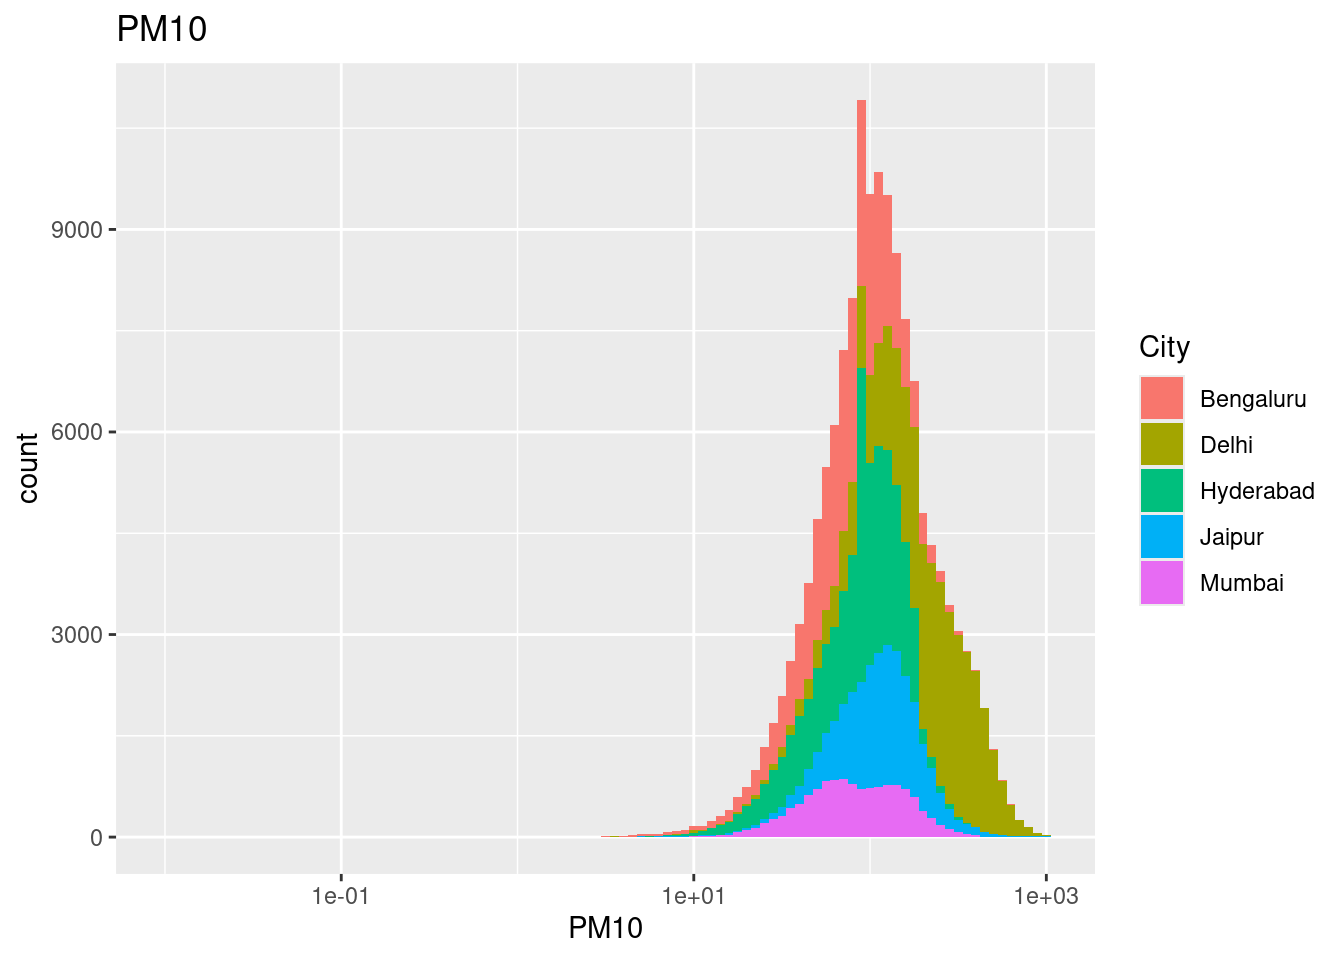
\includegraphics[width=0.7\textwidth]{pm10-by-city.png}
    \caption{PM\textsubscript{10} levels by city}
    \label{fig:pm10_by_city}
\end{figure}


\subsection{Time Series Analysis}

We analyzed whether the time of year affects pollution levels. Although we only present the graph for O\textsubscript{3} pollution, all pollutants exhibit similar behavior: pollution levels tend to be lower during the summer months, from July to September.

\begin{figure}[H]
    \centering
    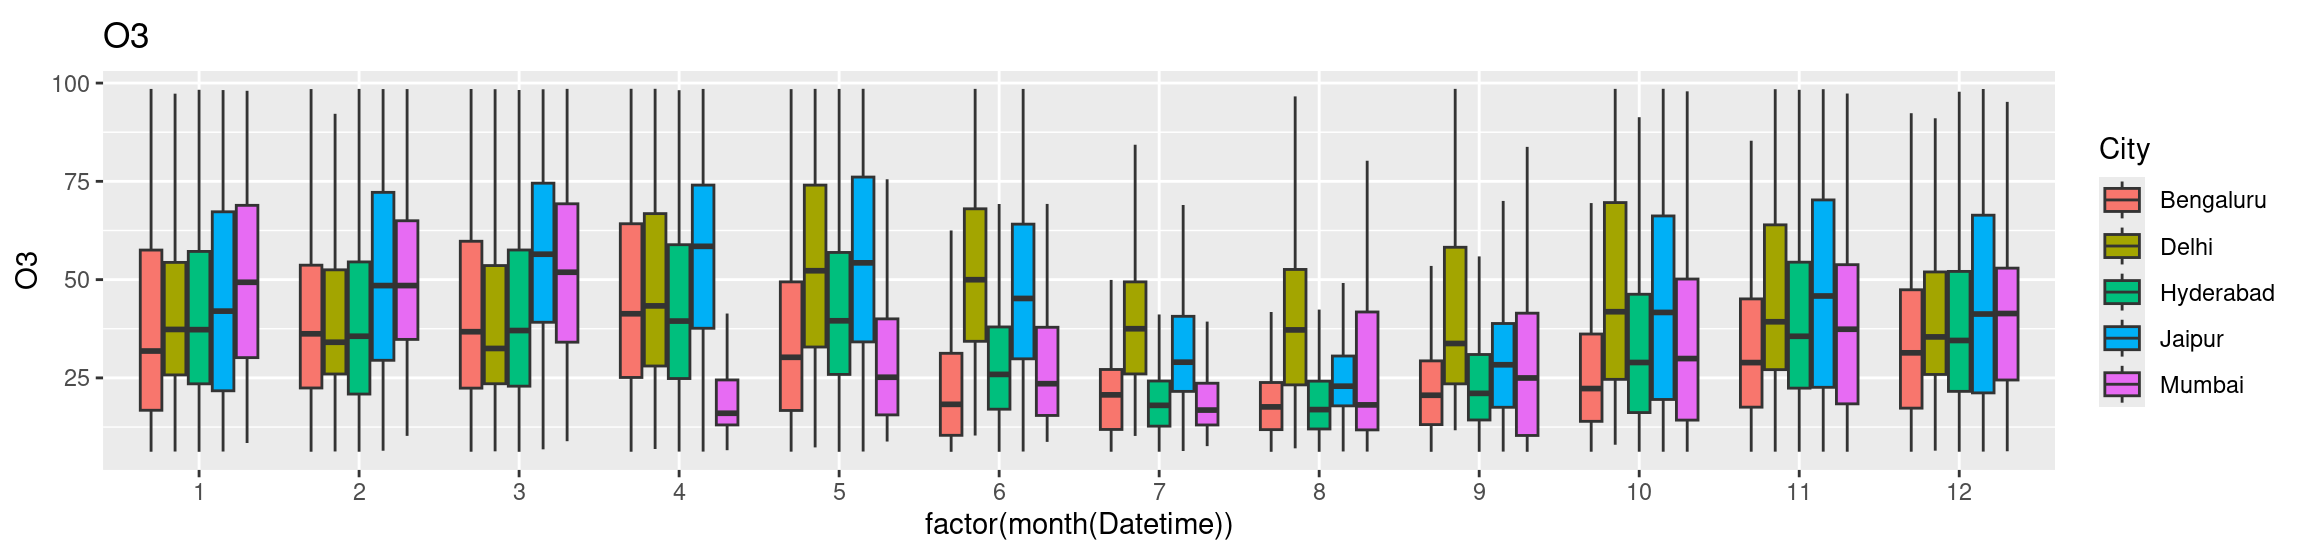
\includegraphics[width=0.7\textwidth]{o3-by-month.png}
    \caption{O\textsubscript{3} levels by month}
    \label{fig:o3_by_month}
\end{figure}

\subsection{Correlation Analysis}

We conducted a correlation analysis to examine the relationships among the weather variables and between the features and response variables.

First, we calculated the correlation matrix for the weather variables:

\begin{figure}[H]
    \centering
    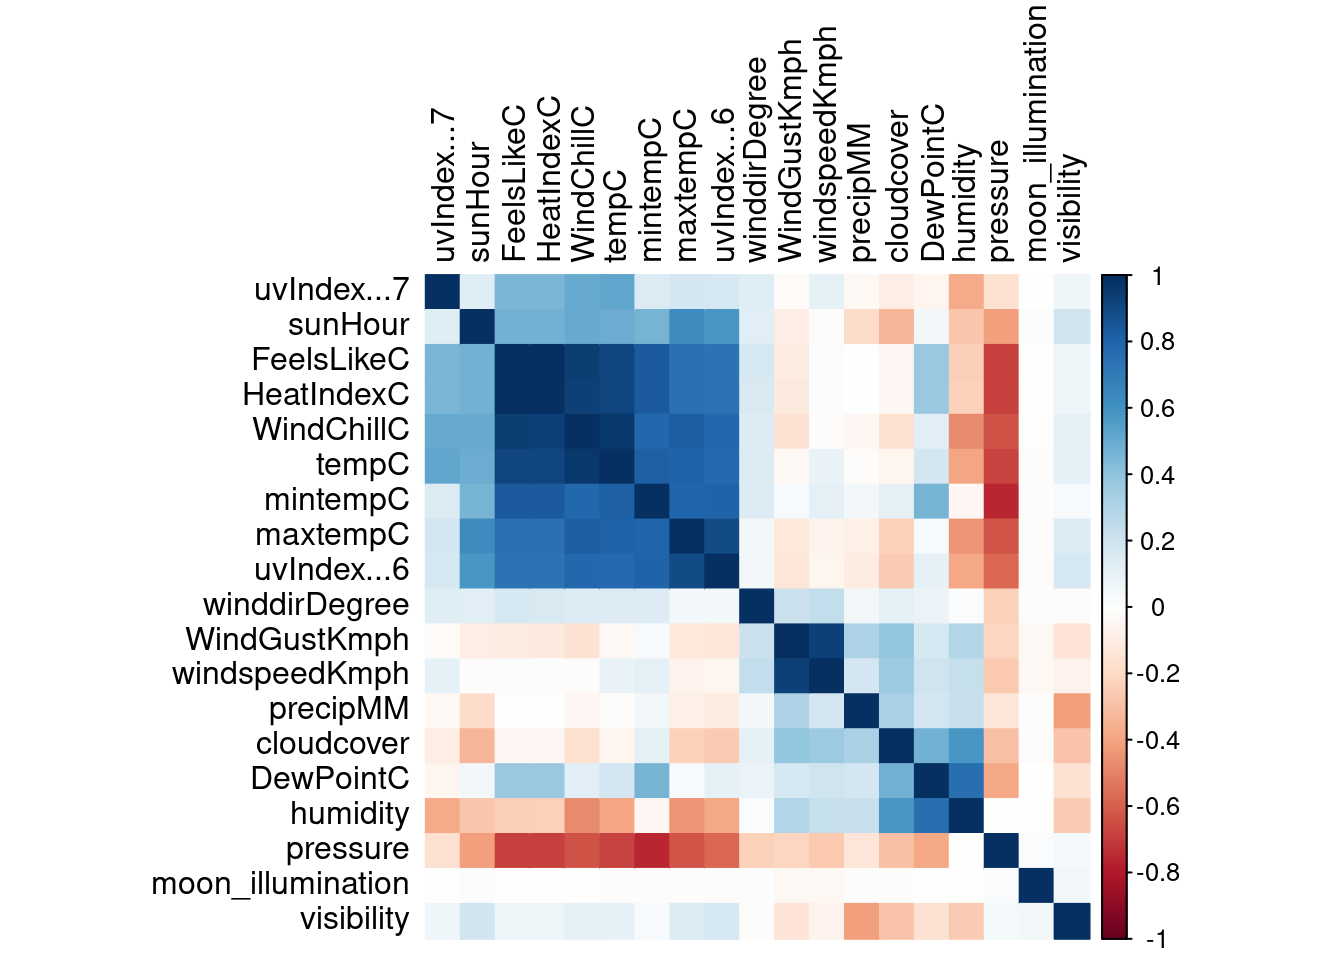
\includegraphics[width=0.7\textwidth]{correlation-matrix.png}
    \caption{Correlation matrix of weather variables}
    \label{fig:correlation_matrix}
\end{figure}

\textbf{Observations:}

The correlation matrix (Figure~\ref{fig:correlation_matrix}) shows that some weather variables are highly correlated with each other. To avoid multicollinearity, we decided to remove variables such as \textit{FeelsLikeC}, \textit{HeatIndexC}, \textit{WindChillC}, \textit{minTempC}, and \textit{maxTempC}, which are highly correlated with \textit{tempC} and are derived from combinations of temperature, humidity, and wind speed. Similarly, \textit{humidity} is correlated with \textit{DewPointC}, and certain UV index variables are highly correlated.

Next, we analyzed the correlation between features and response variables:

\begin{lstlisting}[language=R]
feature_vars <- c(
    "sunHour", "uvIndex", "moon_illumination",
    "DewPointC", "WindGustKmph", "cloudcover", "humidity",
    "precipMM", "pressure", "tempC", "visibility", "winddirDegree", "windspeedKmph"
)

# Calculate the correlation matrix
correlation_matrix <- cor(
    data_merged[, response_vars],
    data_merged[, feature_vars],
    use = "pairwise.complete.obs"
)

# Plot the correlation matrix
corrplot(
    correlation_matrix,
    method = "color",
    tl.col = "black"
)
\end{lstlisting}

\begin{figure}[H]
    \centering
    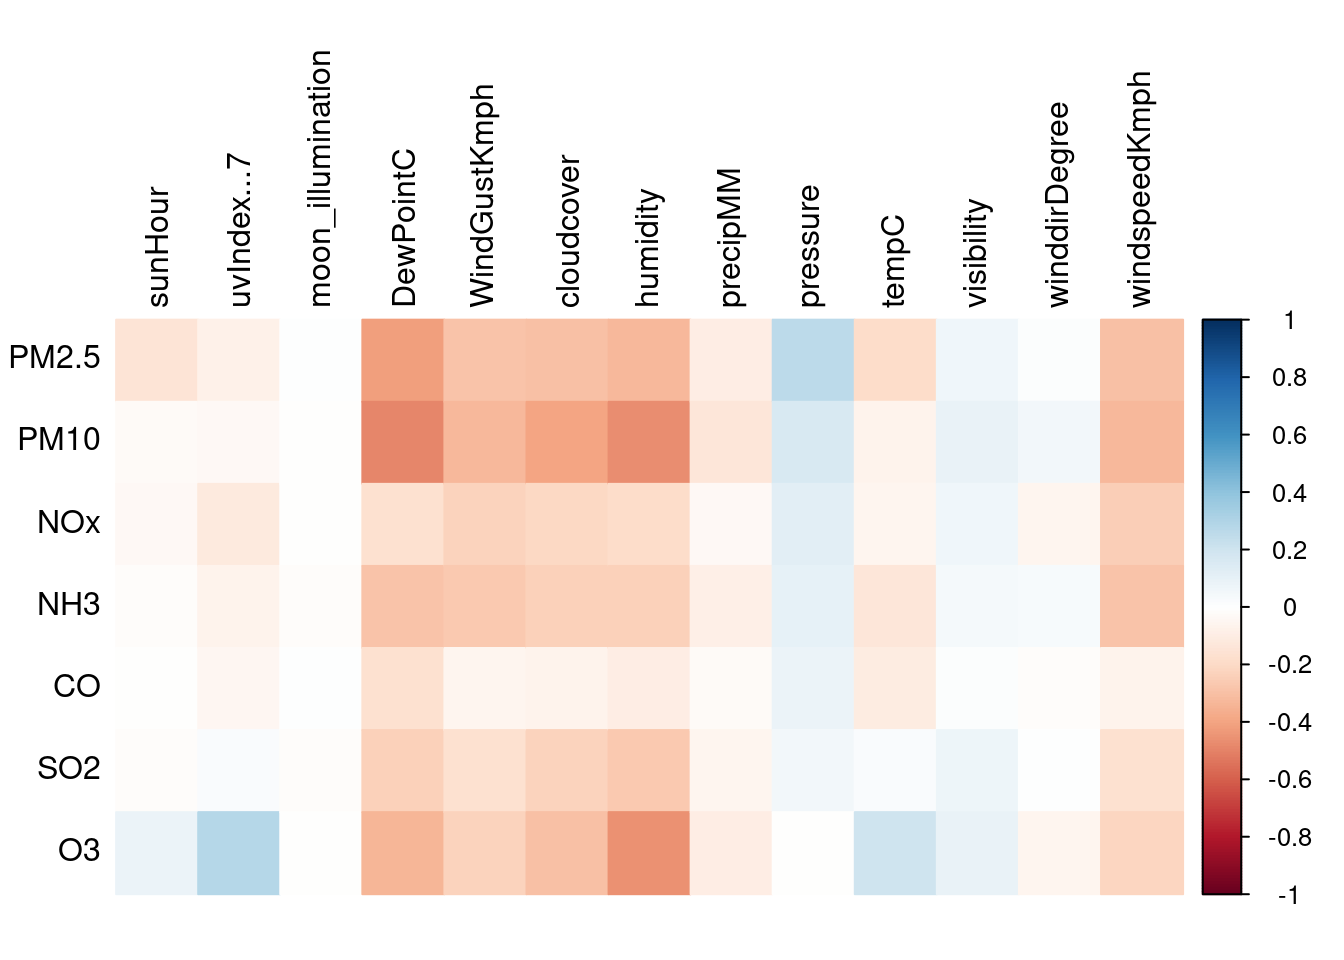
\includegraphics[width=0.7\textwidth]{feature-response-correlation.png}
    \caption{Correlation between features and response variables}
    \label{fig:feature_response_correlation}
\end{figure}

\textbf{Observations:}

The correlation matrix (Figure~\ref{fig:feature_response_correlation}) indicates that the weather variables are weakly correlated with the response variables. However, since we only used a linear correlation measure, there may be non-linear relationships that are not captured in this analysis.

\newpage



% ---------------------------------------------------------------------------------------
% ---------------------------------------------------------------------------------------
% ---------------------------------------------------------------------------------------



% Acknowledgements should go at the end, before appendices and references


% Manual newpage inserted to improve layout of sample file - not
% needed in general before appendices/bibliography.

\bibliography{references}

% Note: in this sample, the section number is hard-coded in. Following
% proper LaTeX conventions, it should properly be coded as a reference:

%In this appendix we prove the following theorem from
%Section~\ref{sec:textree-generalization}:



\end{document}
